\chapter{Measurements}\label{chap:measurements}

In order to test the detector and crystal response, multiple electronic setups were used to obtain spectra from calibrated sources. This chapter summarizes the most important measurements achieved while testing the CosmicWatch, showcasing some features that are yet to be understood. It is important to note that for every measured spectrum a background radiation measurement was also performed and all calibrations were made while subtracting the background. In the plots, sometimes the background is presented to showcase the counts of a spectrum relative to it, when the background is not included in the plot it means that it has been subtracted from that specific spectrum.

\section{CosmicWatch electronics}\label{sec:CW_measurements}

\subsection{ADC shortcomings}\label{sec:ADC_shortcomings}

\subsubsection{Resolution}

\begin{figure}
  \centering
  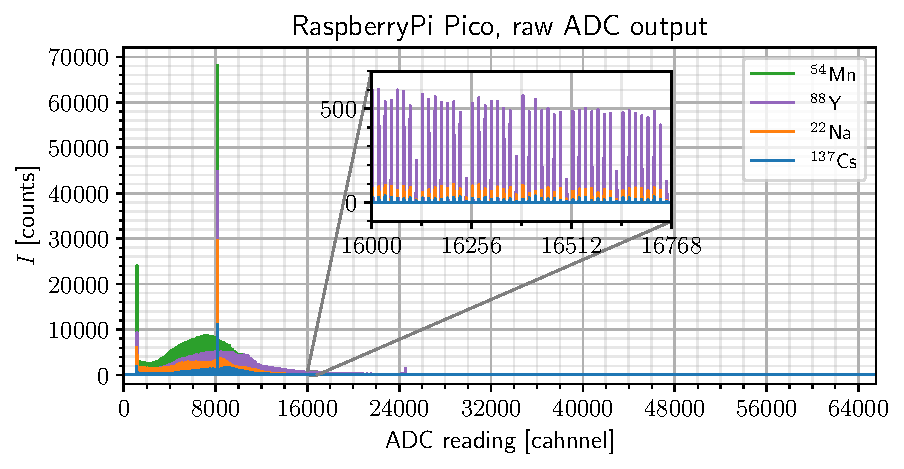
\includegraphics[width=.98\textwidth]{measurements/CW/raw_adc.pdf}
  \caption{\label{fig:CW_raw}Histogram of ADC reading per channel, showcasing some odd features in the ADC.}
\end{figure}

As specified in the RP2040 datasheet \cite[sec.~4.9]{datasheet2024rp2040}, the RaspberryPi Pico has a 12-bit ADC, which means that the 0 to 3.3 \unit{\V} range corresponds to $2^{12}=4096$ channels. Figure \ref{fig:CW_raw} shows a histogram of ADC readings taken with \texttt{spectra.py} (Ap. \ref{sec:spectra.py}), this histogram shows, however, that the ADC outputs data well above 4096, this happens because, as mentioned in the \href{https://docs.micropython.org/en/latest/library/machine.ADC.html#machine.ADC}{MicroPython documentation for the ADC class}, in the function \texttt{ADC.read\_u16} ``the return value represents the raw reading taken by the ADC, scaled such that the minimum value is 0 and the maximum value is 65535.'' This explains why there are so many channels with zero counts in the inset of Fig. \ref{fig:CW_raw}. By rescaling the ADC output to twelve bits we get the data shown in Fig. \ref{fig:CW_scaled}, where the number of channels was therefore reduced from $2^{16}$ to $2^{12}$, thus removing the channels where there were zero counts recorded.

One important issue represented in the inset of Fig. \ref{fig:CW_scaled} is the periodic drop in counts every 8 channels for all measurements, while channel 512 presents an extremely high number of events. The real number of channels in the ADC is important since it determines the resolution of our analog reader, otherwise known as the Least Significant Bit (LSB), which determines the smallest variation in the input signal that the ADC can recognize, the LSB of our ADC can be approximated as shown in equation \eqref{eq:LSB},
\begin{equation}\label{eq:LSB}
  1~\text{LSB} = \frac{\text{V}_\text{REF}}{2^N} = \frac{3.3 \unit{\V}}{2^{12}} \approx 805~\unit{\micro\V}
\end{equation}
this means that ideally, every channel should cover an 805 \unit{\micro\V} range, however, that is not the case in our hardware. The Integral Non-Linearity (INL) and Differential Non-Linearity (DNL) determine the actual resolution of each channel and therefore the ADC response, in this case, we are especially worried about the DNL, Fig. \ref{fig:RP2040_DNL} shows the DNL of every channel in the Pico's ADC. In simple terms, if a channel has a DNL$<0$ its actual LSB will be smaller than the expected value. Channels 512, 1536, 2560, and 3584 are therefore important to notice, their extremely high DNL values mean that they cover a wider voltage range (at 512, DNL$~\approx9$, therefore LSB$(512)=(1+9)$LSB$~\approx 8.05$ \unit{\m\V}), this explains the sudden spike in counts at 512 and the small peak at 1536 in Fig. \ref{fig:CW_scaled}. With this in mind, an approximation of the number of events expected with LSB$~=1$ can be obtained if we divide it by $1+~$DNL (this has been done for all spectra shown from now on that have been measured with the PICO's ADC). From Fig. \ref{fig:RP2040_DNL} it is also clear that there are no significant drops in the DNL every 8 channels, which leaves open the question about the periodic lower counts discussed earlier.

\begin{figure}
  \centering
  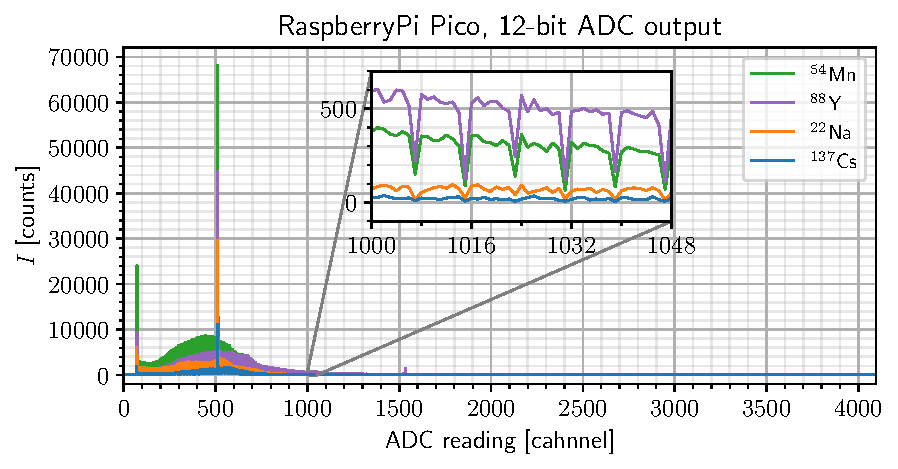
\includegraphics[width=.98\textwidth]{measurements/CW/scaled_raw_adc.pdf}
  \caption{\label{fig:CW_scaled}Histogram of ADC reading per channel, rescaled to 12-bits.}
\end{figure}

\begin{figure}
  \centering
  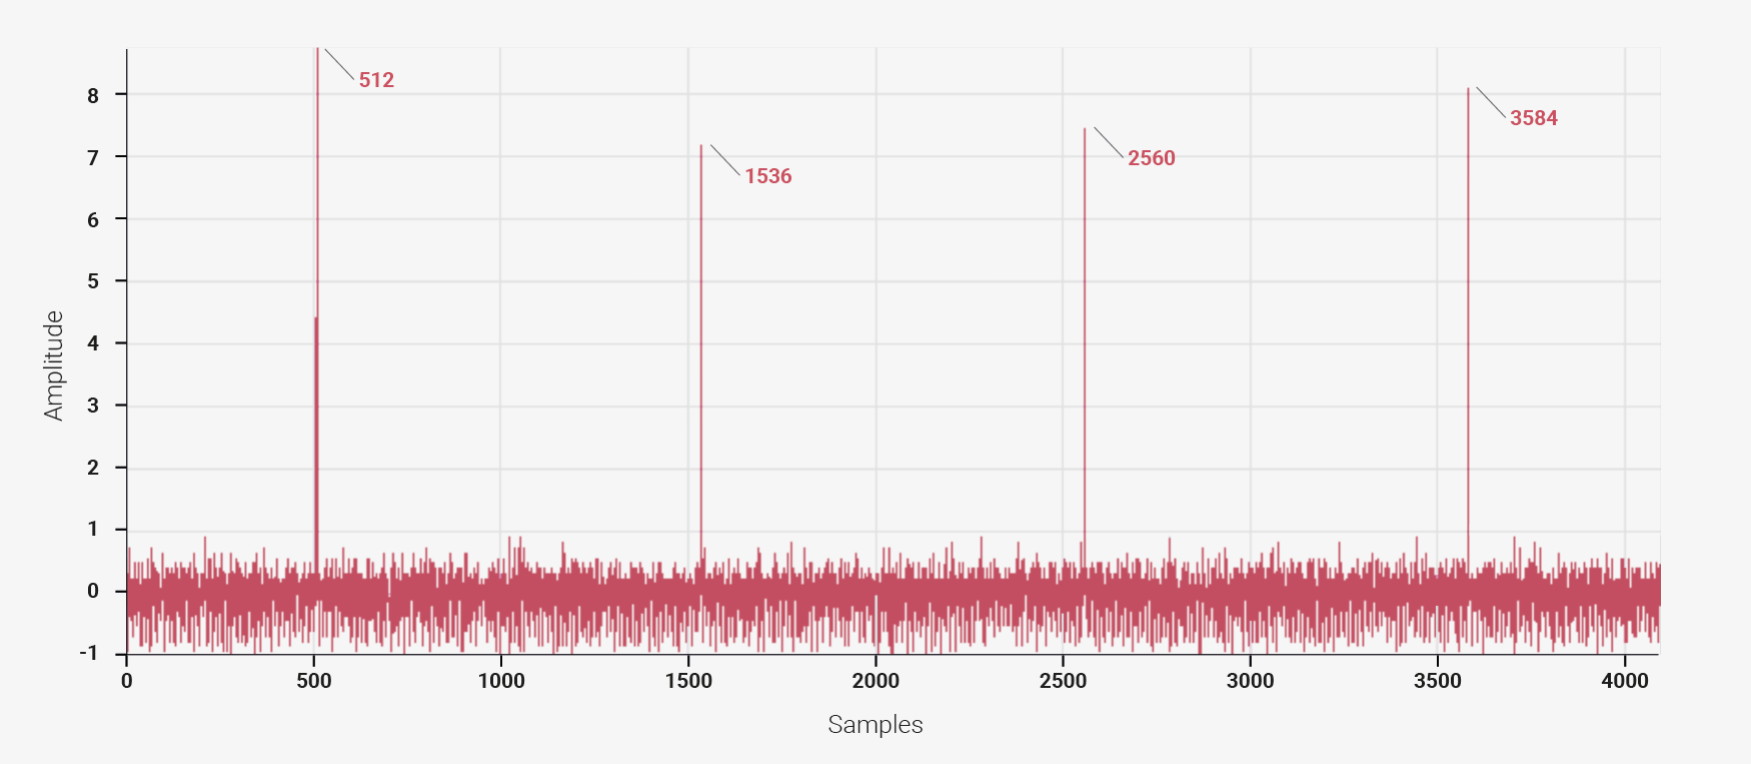
\includegraphics[width=.98\textwidth]{measurements/CW/RP2040_DNL.png}
  \caption{\label{fig:RP2040_DNL}RP2040 ADC Differential Non-Linearity, taken from \cite{datasheet2024rp2040}.}
\end{figure}

The Pico's documentation \cite{datasheet2024RpPico} suggests some changes that can be done to the Pico board that may improve resolution, like reducing the voltage reference (currently set at 3.3V), since this would make the LSB smaller and would take better advantage of our 12-bit resolution.

\subsubsection{Response time}

\begin{figure}[H]
  \centering
  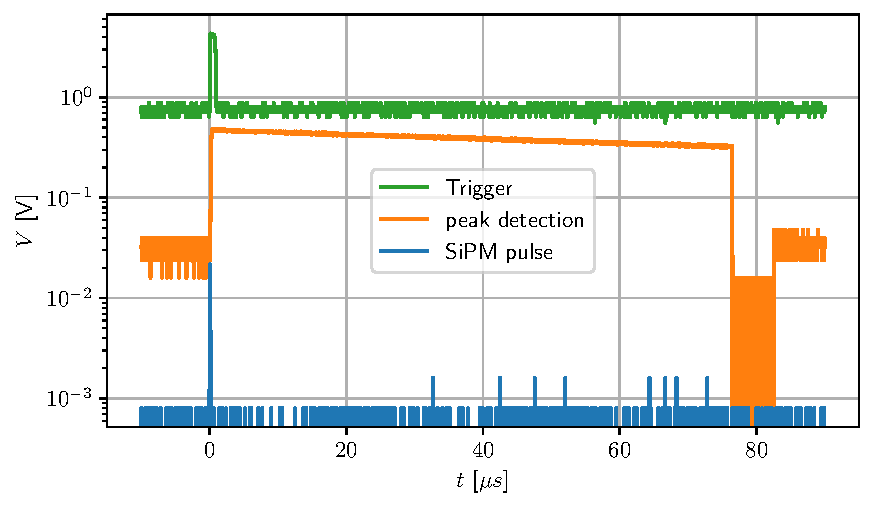
\includegraphics[width=\textwidth]{measurements/CW/Trigger_reset.pdf}
  \caption{\label{fig:measurement_speed}Trigger and measurement time delay after a SiPM pulse.}
\end{figure}

In an attempt to achieve the fastest response possible after a SiPM pulse is sent to the peak detector, an interrupt routine (\texttt{read\_ADC} in \texttt{run.py}) was used to stop all processes and focus on reading the ADC, this is supposed to ensure that the Pico's ADC would read the peak detected signal and the capacitor would be discharged in the shortest time, preventing event loses and pileup with other incoming pulses. 

Figure \ref{fig:measurement_speed} showcases the delay after an incoming SiPM pulse has been detected and processed by the detector, it can be seen that the peak detector's capacitor is discharged by the TriggerReset pin about 76 \unit{\micro\s} after the detector is triggered, this means that the ADC reading could have happened at any moment in that time window. The difference in voltage in the peak detected signal at its maximum and right before the capacitor is discharged is about 176 \unit{\mV}, according to our theoretical LSB, this voltage drop represents a 218 channel difference in the ADC reading.

Increasing the time response could greatly improve the detector's resolution since it would minimize the time delay between incoming pulses and ADC readings, therefore decreasing the error between the recorded value and the real amplitude of the peak-detected signal.

\subsection{Measured spectra}

\begin{figure}[H]
  \centering
  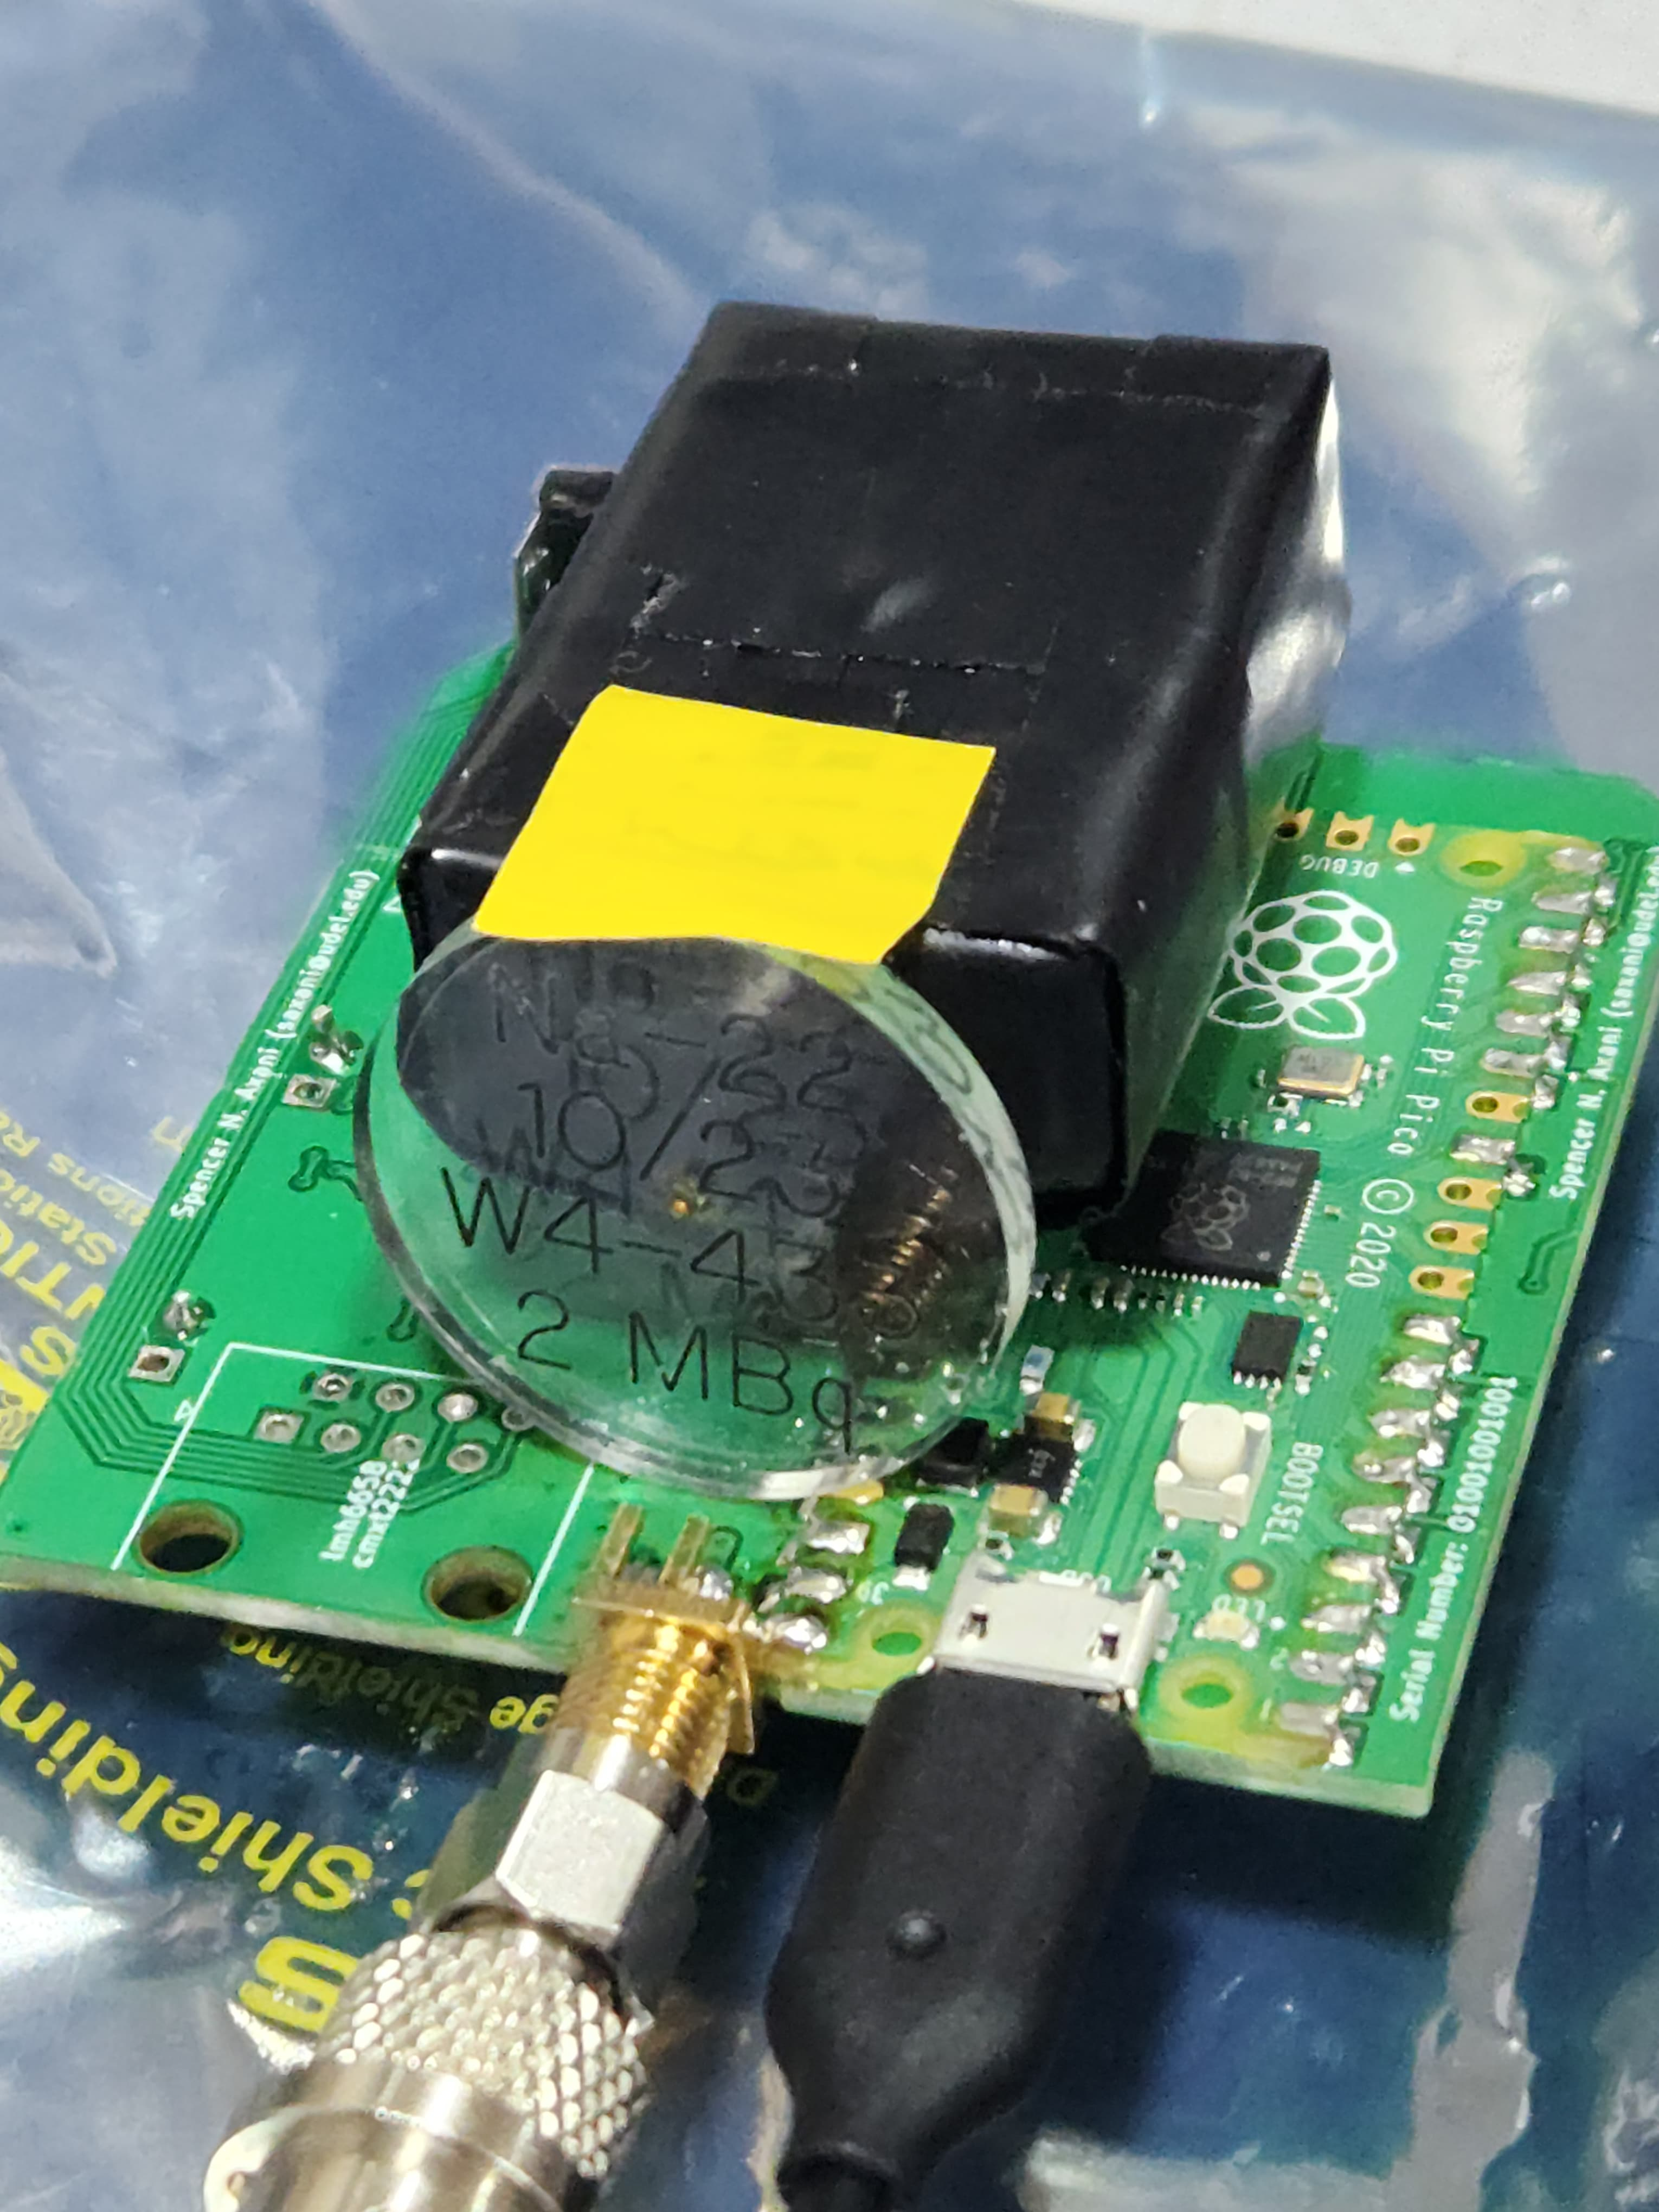
\includegraphics[width=.25\textwidth]{measurements/Source_position.jpg}
  \caption{\label{fig:source_position}Radioactive source positioning relative to the detector. In this picture the transparent disc corresponds to a $^{22}$Na source, which has been held in place by tapping it to the detector.}
\end{figure}

Figure \ref{fig:source_position} shows how the radioactive sources were positioned relative to the detector, it is done this way for two reasons: first, it ensures the gamma rays will have a longer travel path inside the crystal, and second, the small distance seems to produce the best results for low activities, such as those of Manganese, Yttrium, and Cesium, on the other hand, the Sodium source was placed 15 \unit{\cm} away from the detector due to its large activity, since moving it closer only increased Compton counts, although a more thorough analysis could be made in order to find an optimum source position.

Figure \ref{fig:CW_spectra} shows the spectra obtained for four different calibrated sources (the same used while testing the CosmicWatch with NIM modules in Sec. \ref{sec:NIM_modules}) while running the \texttt{spectra.py} script on the Pico for one hour. These spectra take into account the ADC shortcomings showcased in Sec. \ref{sec:ADC_shortcomings}, therefore, the channels range from 0 to 4095, the periodically low counts were ``erased'' by grouping the data every 8 channels, and the large DNL in channels 511 and 1536 was removed by taking the average of the previous and next channel. 

Contrary to the spectra shown in sections \ref{sec:RTO6} and \ref{sec:NIM_modules}, in this case, not all of the photopeaks cover enough channels to fit a gaussian to them, this was only possible for Sodium and Cesium, as showcased in Fig. \ref{fig:CW_spectra}. In the case of Manganese and Yttrium, we can only estimate the centroid to lie at the channel with the most counts in their respective photopeaks, which means that it will have an 8-channel error due to the channel-grouping discussed earlier, doing this we get the calibration shown in Fig. \ref{sfig:CW_LYSO_calibration}.

\begin{figure}[H]
  \begin{subfigure}[t]{0.48\textwidth}
    \centering
    \includegraphics[width=\textwidth]{measurements/CW/22Na.pdf}
    \caption{\label{sfig:CW_22Na}$^{22}$Na, $A=1697.320$ kBq.}
  \end{subfigure}
  \hfill
  \begin{subfigure}[t]{0.48\textwidth}
    \centering
    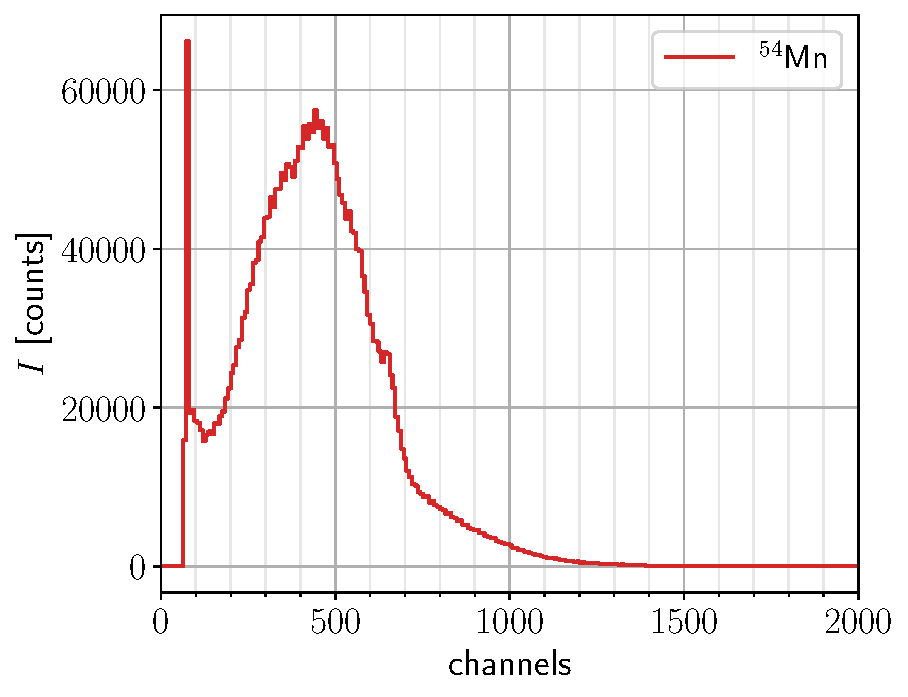
\includegraphics[width=\textwidth]{measurements/CW/54Mn_1.pdf}
    \caption{\label{sfig:C2_54Mn}$^{54}$Mn, $A=623.108$ kBq.}
  \end{subfigure}
  \medskip
  \begin{subfigure}[t]{0.48\textwidth}
    \centering
    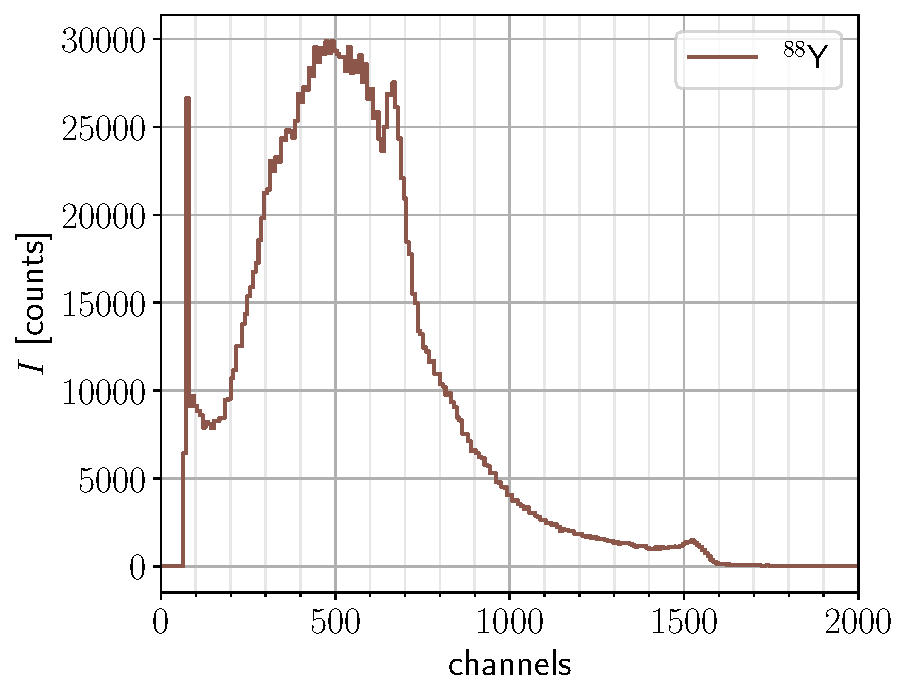
\includegraphics[width=\textwidth]{measurements/CW/88Y_1.pdf}
    \caption{\label{sfig:CW_88Y}$^{88}$Y, $A=251.980$ kBq.}
  \end{subfigure}
  \hfill
  \begin{subfigure}[t]{0.48\textwidth}
    \centering
    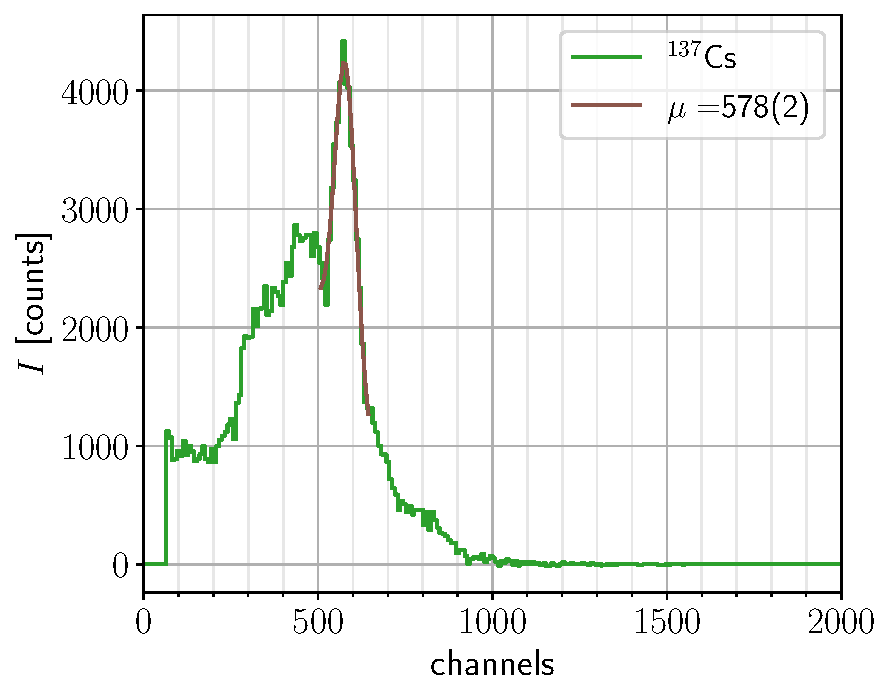
\includegraphics[width=\textwidth]{measurements/CW/137Cs.pdf}
    \caption{\label{sfig:CW_137Cs}$^{137}$Cs, $A=23.139$ kBq.}
  \end{subfigure}
  \caption{\label{fig:CW_spectra}Spectra measured with the Raspberry Pi Pico using the \texttt{spectra.py} script found in Appendix \ref{sec:spectra.py}.}
\end{figure}

As mentioned in subsection \ref{sec:Non-linearity}, the detector's response to variations in SiPM pulse amplitudes is not linear, making necessary the use of an eleven-degree polynomial to represent the peak detector's behavior. Since it was only possible to measure four gamma-ray peaks, it is not possible to use the polynomial calibration showcased in \ref{fig:nonlinearity}, it is for this reason that we have limited our calibration to a linear fit. The lack of a true representation of the detector's nonlinearity is most likely the reason why we find negative energy values in Figure \ref{sfig:CW_joint_spectra}.

Since it was not possible to perform a gaussian fit for all peaks, we can not show an FWHM versus energy comparison which would provide a clear picture of the detector's resolution. Instead, we will have to conform with just the energy resolution at 511 keV, which in this case is 36.5$\%$. Further work needs to be done to increase resolution, some possible alternatives are explored in Chapter \ref{chap:future}.

\begin{figure}[H]
  \begin{subfigure}[t]{\textwidth}
    \centering
    \includegraphics[width=.98\textwidth]{measurements/CW/LYSO_calibration.pdf}
    \caption{\label{sfig:CW_LYSO_calibration}LYSO calibration from Raspberry Pi Pico data. Obtained by fitting gaussian functions to the main peaks of Sodium and Cesium and taking the channel with the most counts in the photopeaks of Manganese and Yttrium.}
  \end{subfigure}
  \medskip
  \begin{subfigure}[t]{\textwidth}
    \centering
    \includegraphics[width=.98\textwidth]{measurements/CW/Calibrated_spectrum.pdf}
    \caption{\label{sfig:CW_joint_spectra}Calibrated spectrum obtained from the channel-energy conversion shown in \subref{sfig:CW_LYSO_calibration}.}
  \end{subfigure}
  \caption{\label{fig:CW_calibration}Gamma-ray spectra obtained with the CosmicWatch detector.}
\end{figure}

\section{Rohde\&Schwarz RTO6 oscilloscope}\label{sec:RTO6}

\begin{figure}[H]
  \begin{subfigure}[t]{0.48\textwidth}
    \centering
    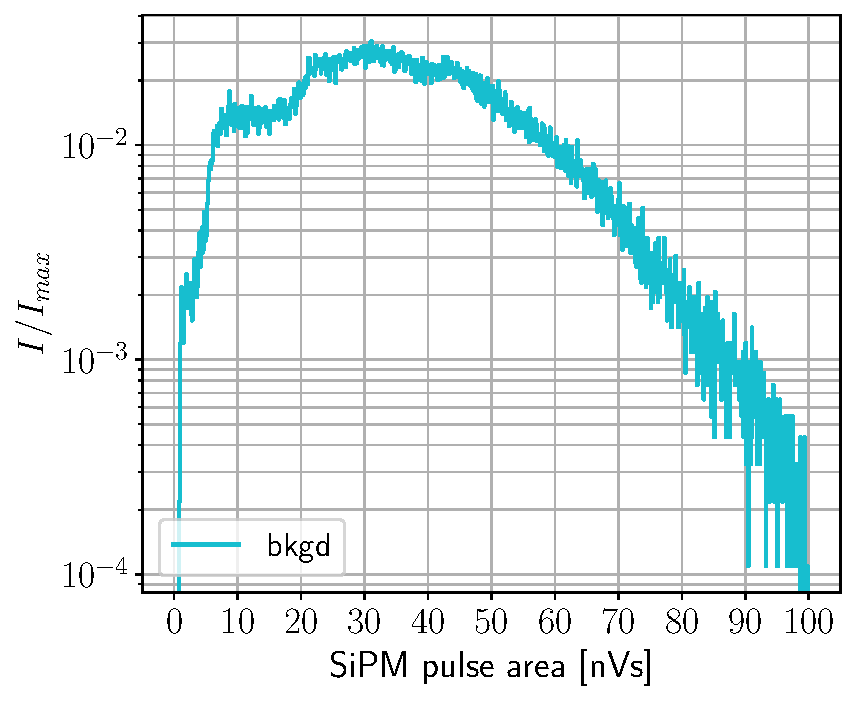
\includegraphics[width=\textwidth]{measurements/RS/teflon-bkgd.pdf}
    \caption{\label{sfig:RS_bkgd}LYSO background.}
  \end{subfigure}
  \hfill
  \begin{subfigure}[t]{0.48\textwidth}
    \centering
    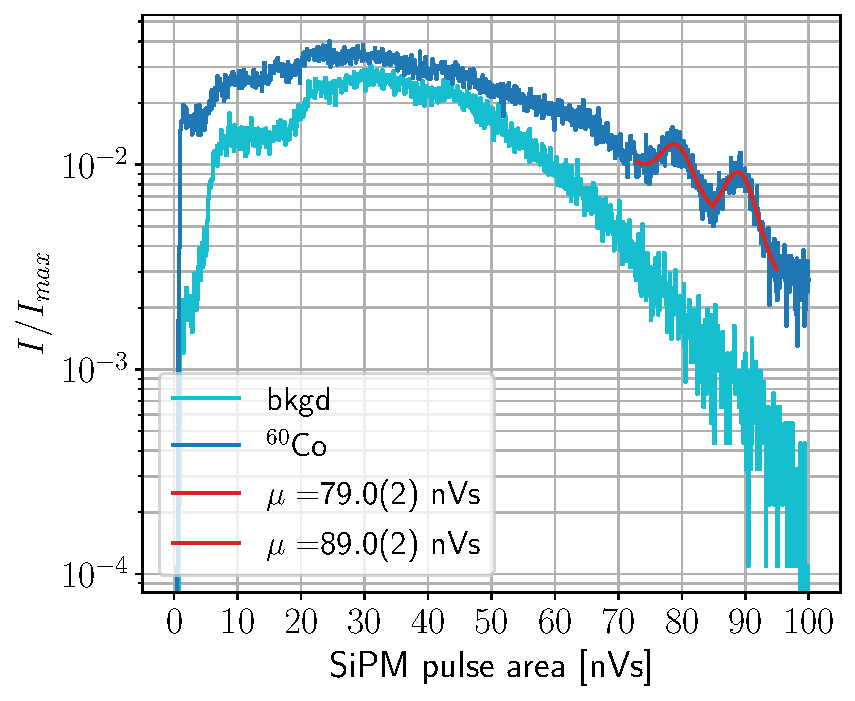
\includegraphics[width=\textwidth]{measurements/RS/teflon-side-Co60.pdf}
    \caption{\label{sfig:RS_60Co}$^{60}$Co.}
  \end{subfigure}
  \medskip
  \begin{subfigure}[t]{0.48\textwidth}
    \centering
    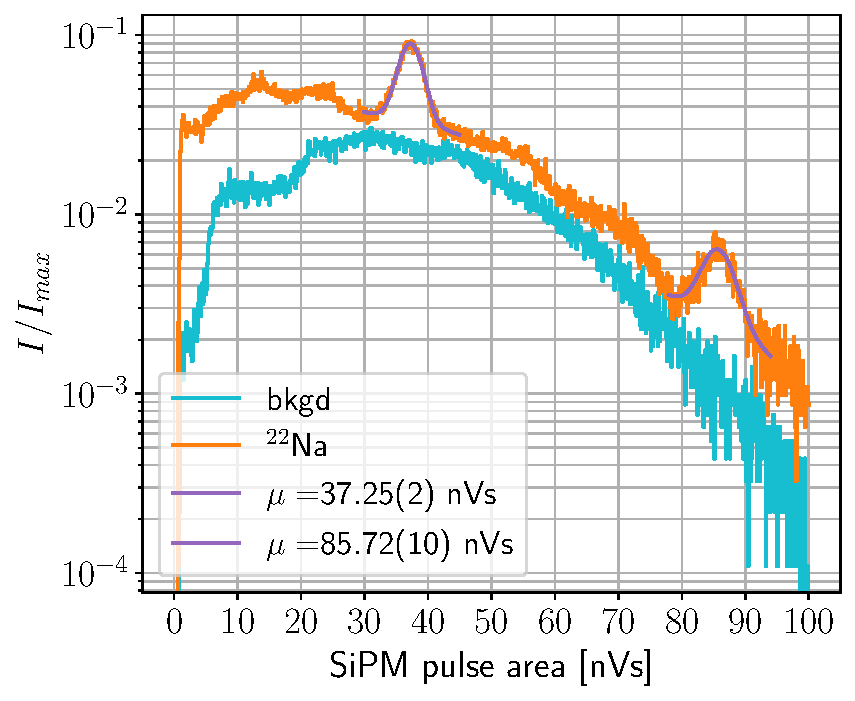
\includegraphics[width=\textwidth]{measurements/RS/teflon-side-Na22.pdf}
    \caption{\label{sfig:RS_22Na}$^{22}$Na.}
  \end{subfigure}
  \hfill
  \begin{subfigure}[t]{0.48\textwidth}
    \centering
    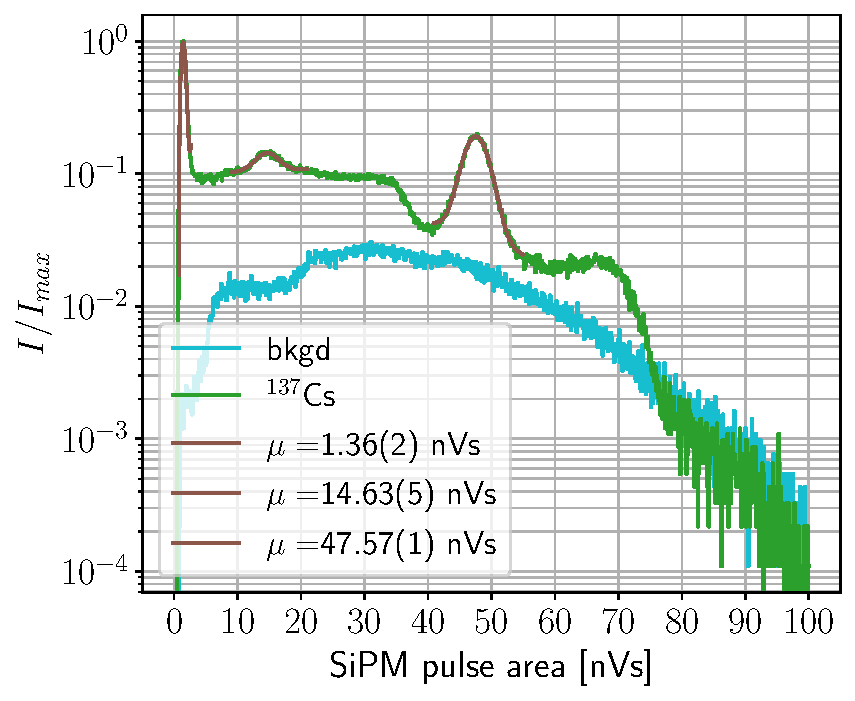
\includegraphics[width=\textwidth]{measurements/RS/teflon-side-Cs137.pdf}
    \caption{\label{sfig:RS_137Cs}$^{137}$Cs.}
  \end{subfigure}
  \caption{\label{fig:RS_spectra}Spectra measured with the histogram functionality of a Rohde\&Schwarz RTO6 oscilloscope. Each graph features the centroid of the Gaussian fitted to each peak.}
\end{figure}

The Rohde\&Schwarz RTO6 oscilloscope was the main troubleshooting tool used to test the detector as a whole. The histogram functionality on the oscilloscope allowed us to also measure spectra from calibrated sources, Figure \ref{fig:RS_spectra} shows the obtained spectra. The $x$ axis measures SiPM pulse areas since the oscilloscope creates histograms based on the area under each SiPM pulse (\textcolor{blue}{blue} signal in Fig. \ref{fig:signal_processing}).

It is important to note here the shape of the background (Fig. \ref{sfig:RS_bkgd}), remembering Figure \ref{fig:LYSO_background}, a sudden increase in intensity should occur at around 290 and 597 \unit{\kilo\eV}, therefore the 511 \unit{\kilo\eV} peak of $^{22}$Na should lie in between these values, while 662 \unit{\kilo\eV} from $^{137}$Cs would lie above the second increase in background counts. These approximations can help us get a notion of what we are seeing in the various spectra illustrated in Fig. \ref{fig:RS_spectra}.

The peak below 10 nVs in $^{137}$Cs is presumed to be caused by x-ray emissions from lower shell electrons filling the space left by internal conversion electrons, this peak is also featured in Figure \ref{fig:Cs137_description}. One important feature in the caesium spectrum is the relatively high intensities in channels above the photopeak (at 47.57(1) nVs according to the gaussian fit), this is not due to LYSO background since these counts greatly exceed the expected background.

Fitting gaussian functions to the main peaks one can get the relation between energy and pulse area (Fig. \ref{sfig:RS_LYSO_calibration_low_peaks}) based on the decay schemes shown in Figure \ref{fig:decay_schemes}. Considering the x-ray and backscattering peaks of $^{137}$Cs, however, seems to cause an overestimation of the energies, as can be seen in Figure \ref{sfig:RS_LYSO_calibrated_spectrum_low_peaks}, where the pair-production peak of sodium, for example, lies at 535.95 keV instead of 511 keV. The calibration shown in Figure \ref{sfig:RS_LYSO_calibration} does not take into account the troublesome peaks of caesium, better estimating high energy peaks, this however results in negative-energy predictions at the lower energy range in the spectrum.

\begin{figure}[H]
  \begin{subfigure}[t]{\textwidth}
    \centering
    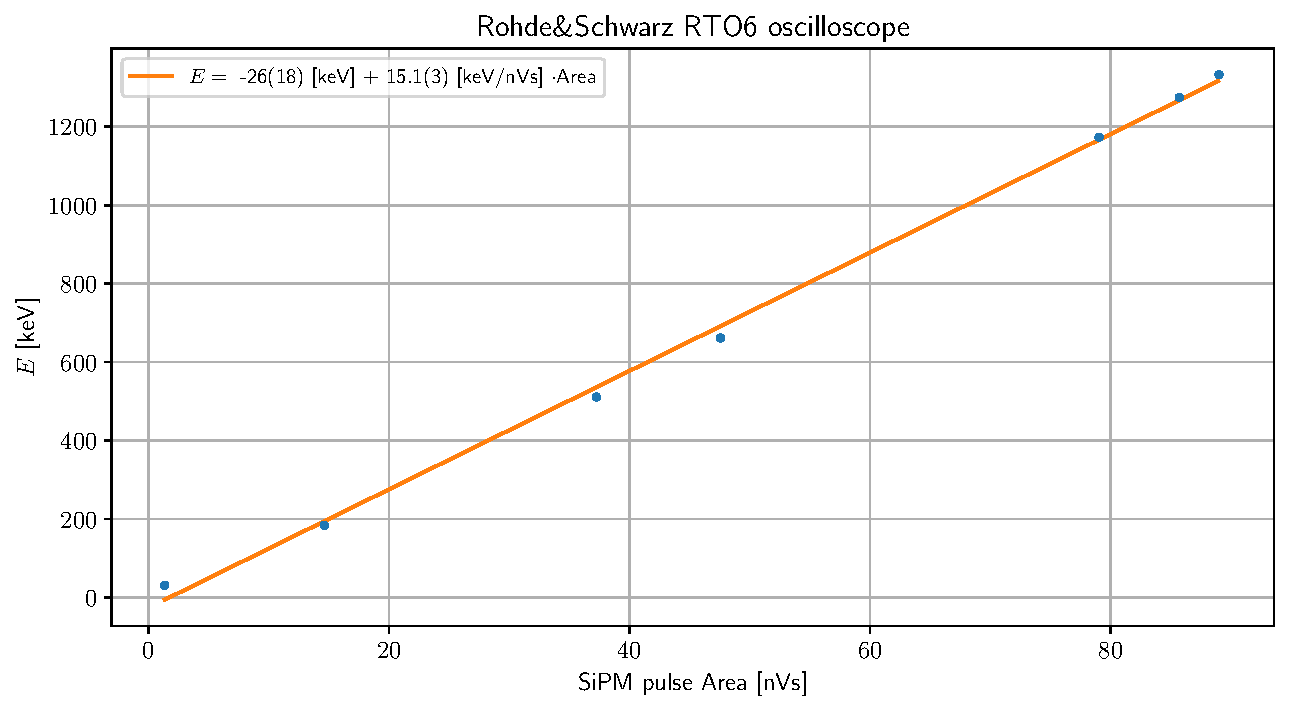
\includegraphics[width=.98\textwidth]{measurements/RS/LYSO_calibration_low_peaks.pdf}
    \caption{\label{sfig:RS_LYSO_calibration_low_peaks}LYSO calibration from Rohde\&Schwarz oscilloscope data. Obtained by fitting gaussian functions to the main peaks shown in Fig \ref{sfig:RS_60Co}, \subref{sfig:RS_22Na}, and \subref{sfig:RS_137Cs}.}
  \end{subfigure}
  \medskip
  \begin{subfigure}[t]{\textwidth}
    \centering
    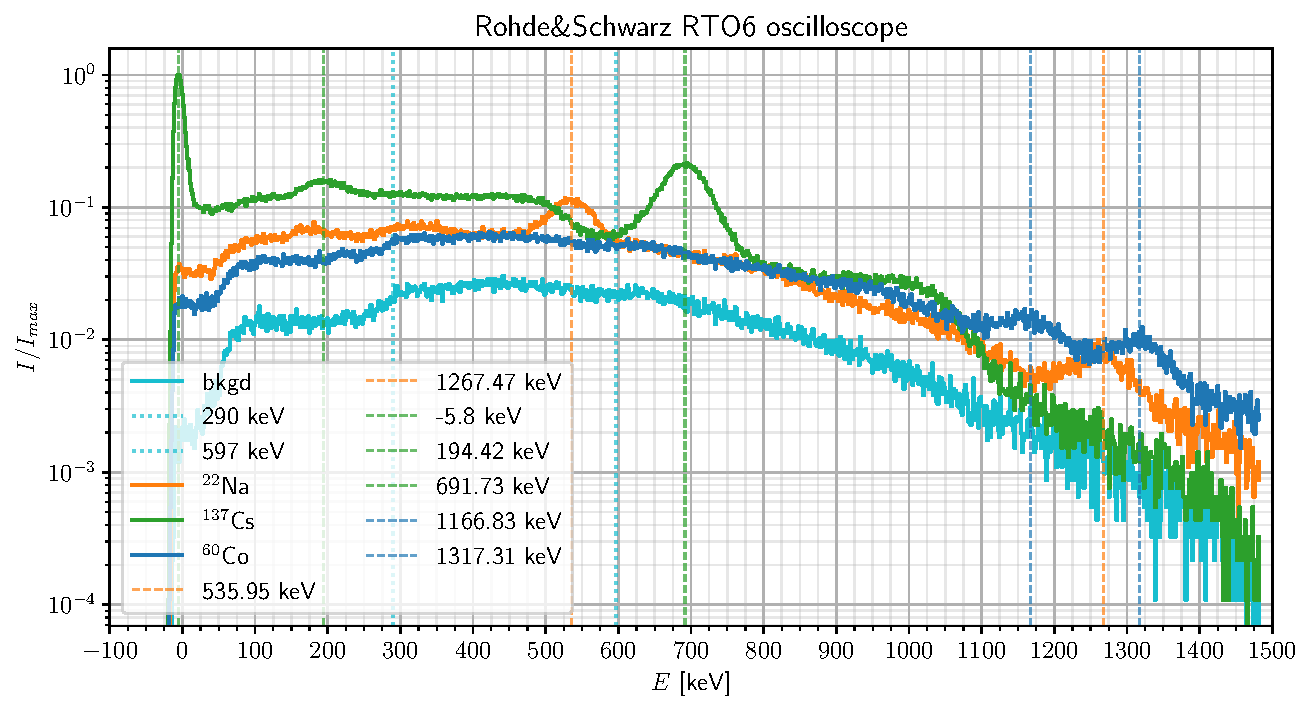
\includegraphics[width=.98\textwidth]{measurements/RS/Calibrated_spectrum_low_peaks.pdf}
    \caption{\label{sfig:RS_LYSO_calibrated_spectrum_low_peaks}Calibrated spectrum obtained from the channel-energy conversion shown in \subref{sfig:RS_LYSO_calibration_low_peaks}.}
  \end{subfigure}
  \caption{\label{fig:RS_low_peaks_calibration}Calibrated spectrum taking into account the x-ray and backscattering peaks of $^{137}$Cs.}
\end{figure}

\begin{figure}[H]
  \begin{subfigure}[t]{\textwidth}
    \centering
    \includegraphics[width=.98\textwidth]{measurements/RS/LYSO_calibration.pdf}
    \caption{\label{sfig:RS_LYSO_calibration}LYSO calibration from Rohde\&Schwarz oscilloscope data. Excluding x-ray and backscattering peaks from \subref{sfig:RS_137Cs}.}
  \end{subfigure}
  \medskip
  \begin{subfigure}[t]{\textwidth}
    \centering
    \includegraphics[width=.98\textwidth]{measurements/RS/Calibrated_spectrum.pdf}
    \caption{\label{sfig:RS_LYSO_calibrated_spectrum}Calibrated spectrum obtained from the channel-energy conversion shown in \subref{sfig:RS_LYSO_calibration}.}
  \end{subfigure}
  \caption{\label{fig:RS_calibration}Calibrated spectrum, ignoring the x-ray and backscattering peaks of $^{137}$Cs.}
\end{figure}

\newpage
In general, the $\chi^2$ results for the multiple fits performed were much better while ignoring the low energies of Cesium, leading us to conclude that this might be optimal, obtaining the final FWHM vs Energy calibration shown in Fig. \ref{fig:RS_FWHM}. This results in an energy resolution of 13.5\% at 511 keV.

\begin{figure}[H]
  \centering
  \includegraphics[width=.98\textwidth]{measurements/RS/FWHM.pdf}
  \caption{\label{fig:RS_FWHM}FWHM as a function of energy from spectra obtained with a Rohde\&Schwarz RTO6 oscilloscope.}
\end{figure}

\newpage
\section{NIM modules}\label{sec:NIM_modules}

In the same way the CosmicWatch was studied with the Rohde\&Schwarz oscilloscope, NIM modules were used to get a LYSO calibration when coupled to the SiPM, this section shows some of the results obtained.

\subsection{Odd features}

While testing the detector response some odd features were found in the measured spectra, they are yet to be understood and present an interesting study case, Figure \ref{fig:NIM_odd_features} showcases some of the spectra obtained that illustrate these anomalies.

$^{54}$Mn, is a monoenergetic source (see Fig. \ref{sfig:54Mn}), producing a peak at 835 \unit{\kilo\eV}, which lies slightly above 662 \unit{\kilo\eV} ($^{137}$Cs), therefore, the peak in channel 259 in Fig. \ref{sfig:NIM_odd_54Mn} should correspond to the gamma emission from Manganese. However, there is again a very high number of events in channels above the photopeak, which is not expected, since 835 \unit{\kilo\eV} is the maximum energy one should see in this spectrum. Aside from this, it is also clear that the shape of this peak does not fully adjust to a gaussian distribution, showing that there is an underlying structure that has not been explained. These odd features can also be seen in $^{137}$Cs.

\begin{figure}[H]
  \centering
  \begin{subfigure}[t]{0.53\textwidth}
    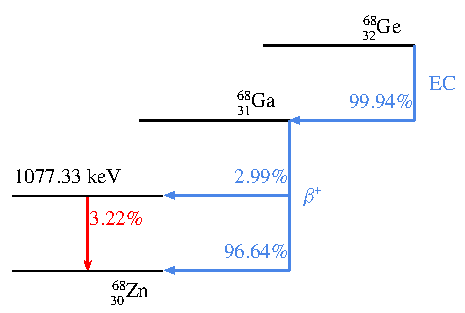
\includegraphics[width=\textwidth]{measurements/68Ge-decay.pdf}
    \caption{\label{sfig:68Ge_decay_scheme}}
  \end{subfigure}
  \begin{subfigure}[t]{0.425\textwidth}
    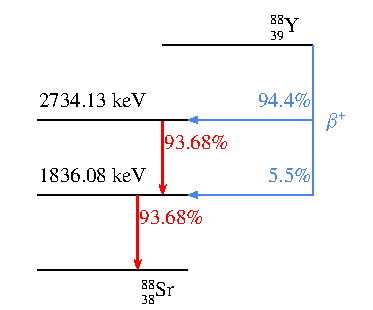
\includegraphics[width=\textwidth]{measurements/88Y-decay.pdf}
    \caption{\label{sfig:88Y_decay_scheme}}
  \end{subfigure}
  \caption{\label{fig:some_decay_schemes}Decay schemes for $^{68}$Ge and $^{88}$Y}
\end{figure}

In principle, $^{68}$Ge should have a spectrum very similar to $^{22}$Na, in this case, however, the decay chain most often ends in a stable state of $^{68}$Zn as illustrated in Fig. \ref{sfig:68Ge_decay_scheme}, this means that the only appreciable peak should lie at 511 \unit{\kilo\eV}, due to pair production from the 1077.33 \unit{\kilo\eV} gamma emission and the subsequent positron annihilation. This agrees with Fig. \ref{sfig:NIM_odd_68Ge}, notably, however, there are very few counts at energies above 511 \unit{\kilo\eV}, which is not the case for the other sources, they present high counts above their respective photopeak. This may be due to the low activity of the source. 

\begin{figure}[H]
  \begin{subfigure}[t]{0.47\textwidth}
    \centering
    \includegraphics[width=\textwidth]{measurements/NIM/odd_features/22Na.pdf}
    \caption{\label{sfig:NIM_odd_22Na}$^{22}$Na, $A=1697.320$ kBq.}
  \end{subfigure}
  \hfill
  \begin{subfigure}[t]{0.47\textwidth}
    \centering
    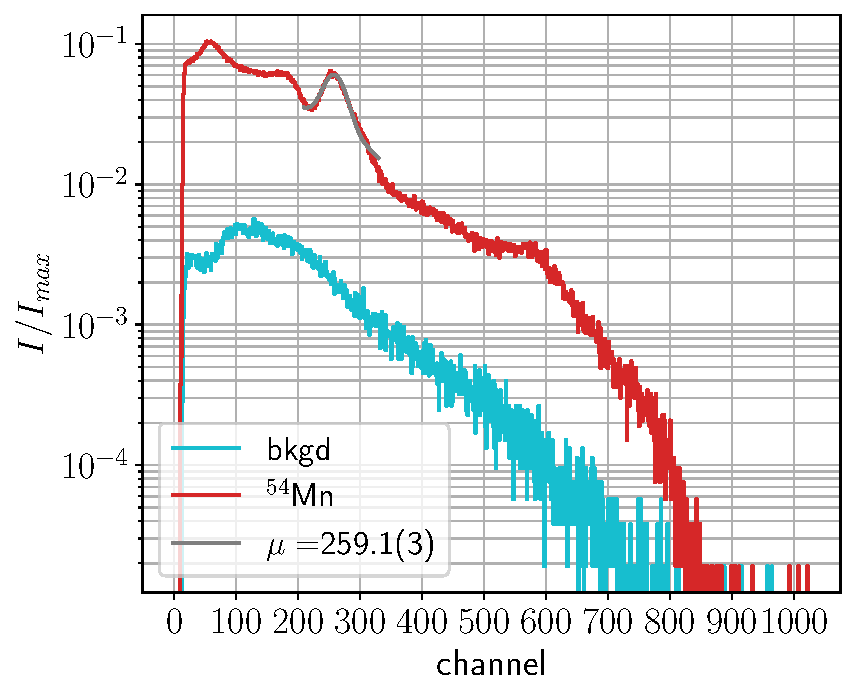
\includegraphics[width=\textwidth]{measurements/NIM/odd_features/54Mn.pdf}
    \caption{\label{sfig:NIM_odd_54Mn}$^{54}$Mn, $A=623.108$ kBq.}
  \end{subfigure}
  \medskip
  \begin{subfigure}[t]{0.47\textwidth}
    \centering
    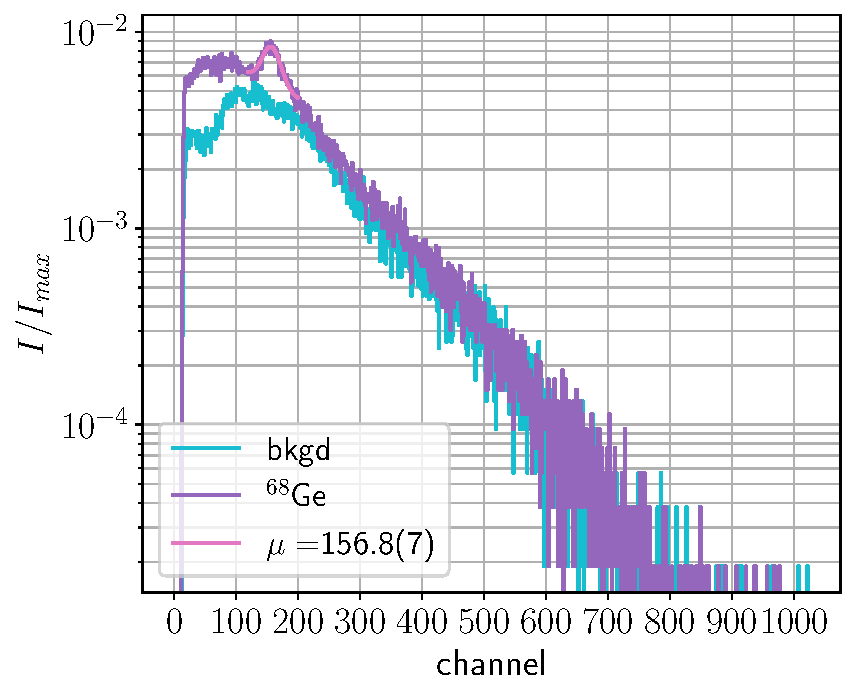
\includegraphics[width=\textwidth]{measurements/NIM/odd_features/68Ge.pdf}
    \caption{\label{sfig:NIM_odd_68Ge}$^{68}$Ge, $A=6.403$ kBq.}
  \end{subfigure}
  \hfill
  \begin{subfigure}[t]{0.47\textwidth}
    \centering
    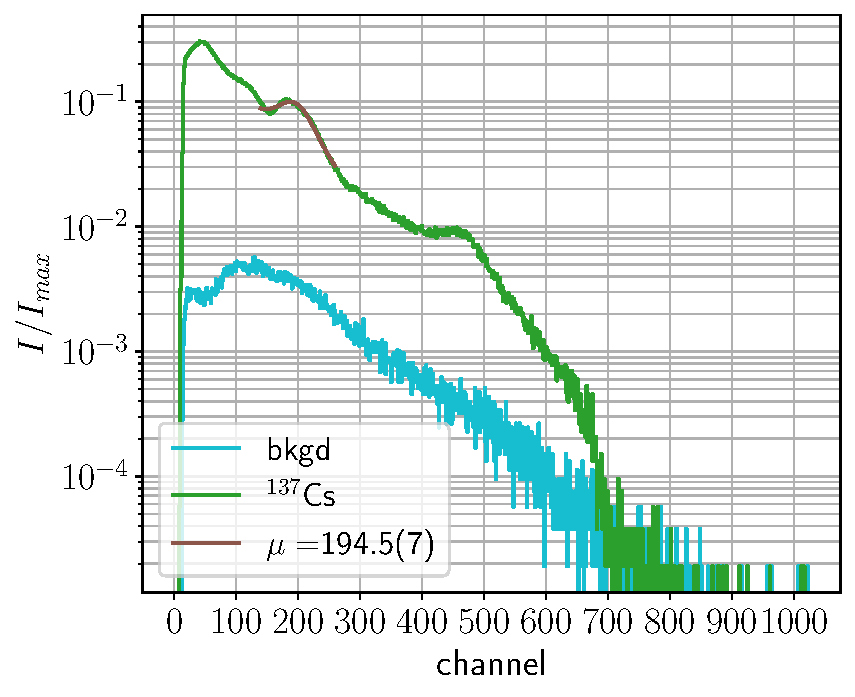
\includegraphics[width=\textwidth]{measurements/NIM/odd_features/137Cs_HA.pdf}
    \caption{\label{sfig:NIM_odd_137Cs}$^{137}$Cs, $A=30790.372$ kBq.}
  \end{subfigure}
  \caption{\label{fig:NIM_odd_features}Spectra measured with a Timing Filter Amplifier and Analog to Digital Converter NIM modules. Each graph features the isotope used, its activity at the time of measurement, and the centroid of the Gaussian fitted to each peak. The $x$ axis gives channels since the ADC creates a histogram based on pulse area. Some odd features can be seen in these spectra, like the large number of counts above the Cesium and Manganese photopeaks.}
\end{figure}

The Cesium spectrum shown in Fig. \ref{sfig:NIM_odd_137Cs} was taken while placing the source 10 cm away from the detector, trying to reduce the count rate due to the large activity of the source, nonetheless, this resulted in an oddly shaped photopeak, and therefore a comparatively large FWHM

%\begin{figure}[H]
%  \centering
%  \includegraphics[width=.98\textwidth]{measurements/NIM/odd_features/FWHM.pdf}
%  \caption{\label{fig:NIM_odd_FWHM}FWHM obtained from gaussian fits to the photo- and positron-annihilation peaks shown in \ref{fig:NIM_odd_features}.}
%\end{figure}

\subsection{Calibration}

Following the goal of this work, multiple spectra were measured trying to find the NIM-modules setup that would optimize energy resolution. As expressed in \cite[sec.~4.4.3]{gilmore2008practical}: ``theory suggests that the lowest noise contribution is found when the integration and differentiation times are made equal. On all modern amplifiers, the shaping time constants are made equal and are controlled by a single selector knob.'' In our case, however, the integration and differentiation times were controlled independently, since we used a Canberra Model 2111 Timing Filter Amplifier \cite{CanberraTFA}. So far, the best results were found while using the OUT setup for both time constants, corresponding to 4 ns of integration time and 160 $\mu$s of differentiation time. 

Even though the FWHM does not vary significantly for different time-constant setups, the OUT configuration produced the most accurate calibrations achieved, obtaining an energy resolution of 25.2\% at 511 keV. Further work needs to be done to better understand the origin of the odd features presented above, this may greatly influence the energy resolution since, as can be seen in the Manganese spectrum, not all the peaks present a truly gaussian form.

\begin{figure}[H]
  \centering
  \includegraphics[width=.98\textwidth]{measurements/NIM/2024-05-24/outD/FWHM.pdf}
  \caption{\label{fig:NIM_FWHM}FWHM obtained from gaussian fits to the photo- and positron-annihilation peaks shown in \ref{fig:NIM_spectra}.}
\end{figure}

It is worth noting the great similarities between Figures \ref{sfig:NIM_54Mn}-\subref{sfig:NIM_88Y} and the features explained in subsection \ref{sec:gammas_in_the_detector}, each showcasing a clear photopeak, Compton edge, and backscattering peak.

\begin{figure}[H]
  \begin{subfigure}[t]{0.47\textwidth}
    \centering
    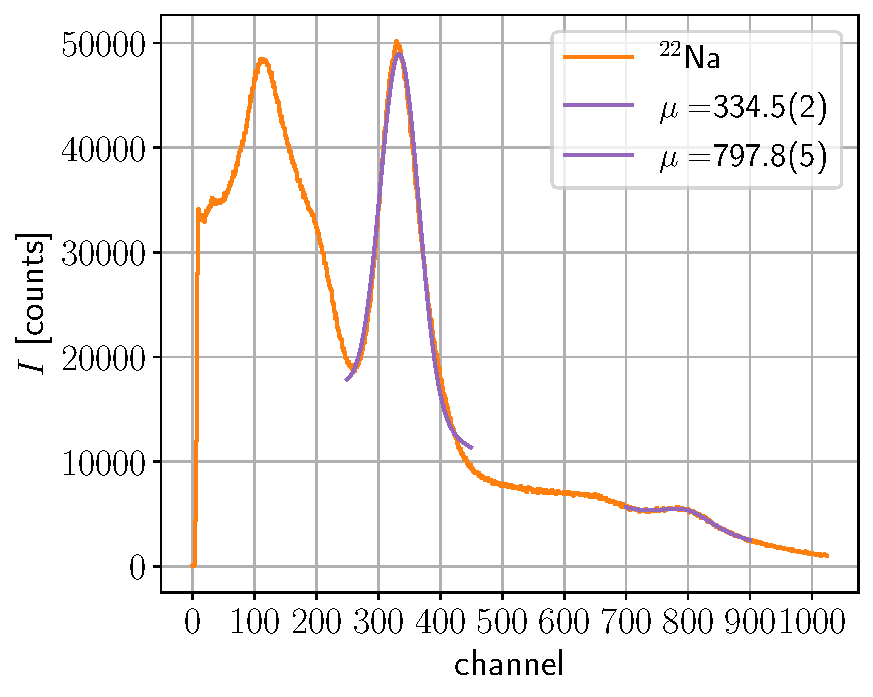
\includegraphics[width=\textwidth]{measurements/NIM/2024-05-24/outD/outD_22Na.pdf}
    \caption{\label{sfig:NIM_22Na}$^{22}$Na, $A=1697.320$ kBq.}
  \end{subfigure}
  \hfill
  \begin{subfigure}[t]{0.47\textwidth}
    \centering
    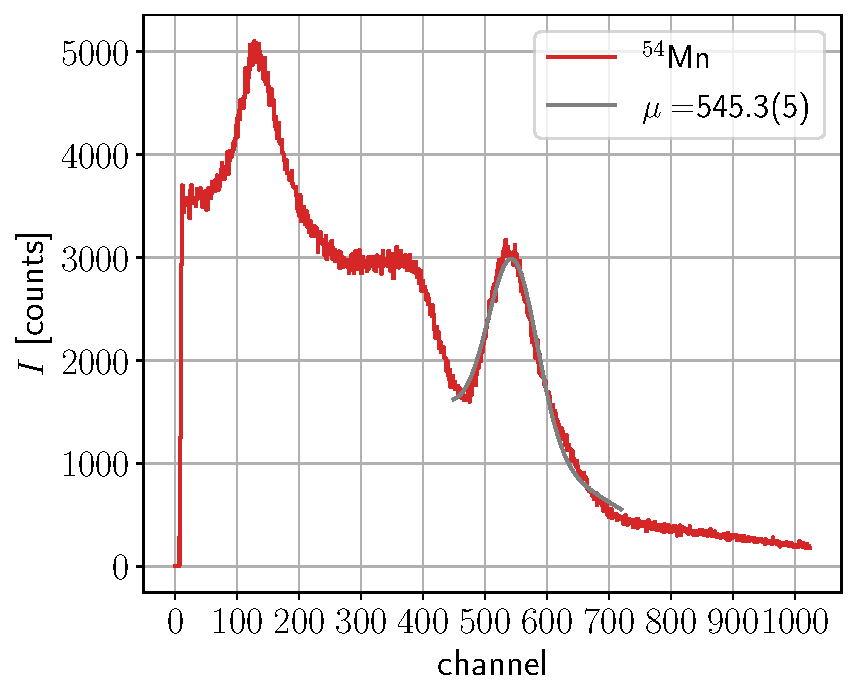
\includegraphics[width=\textwidth]{measurements/NIM/2024-05-24/outD/outD_54Mn.pdf}
    \caption{\label{sfig:NIM_54Mn}$^{54}$Mn, $A=623.108$ kBq.}
  \end{subfigure}
  \medskip
  \begin{subfigure}[t]{0.47\textwidth}
    \centering
    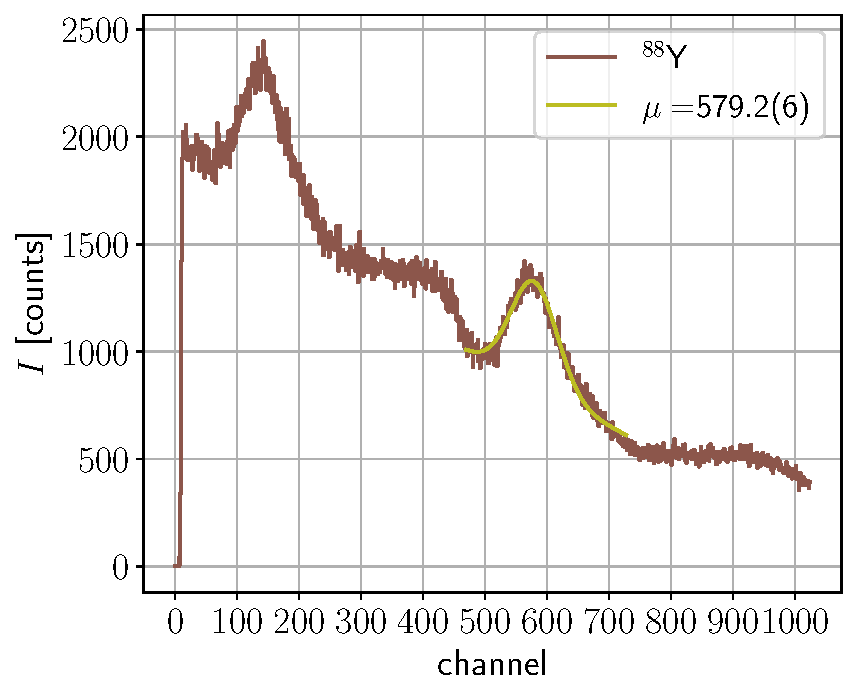
\includegraphics[width=\textwidth]{measurements/NIM/2024-05-24/outD/outD_88Y.pdf}
    \caption{\label{sfig:NIM_88Y}$^{88}$Y, $A=251.980$ kBq.}
  \end{subfigure}
  \hfill
  \begin{subfigure}[t]{0.47\textwidth}
    \centering
    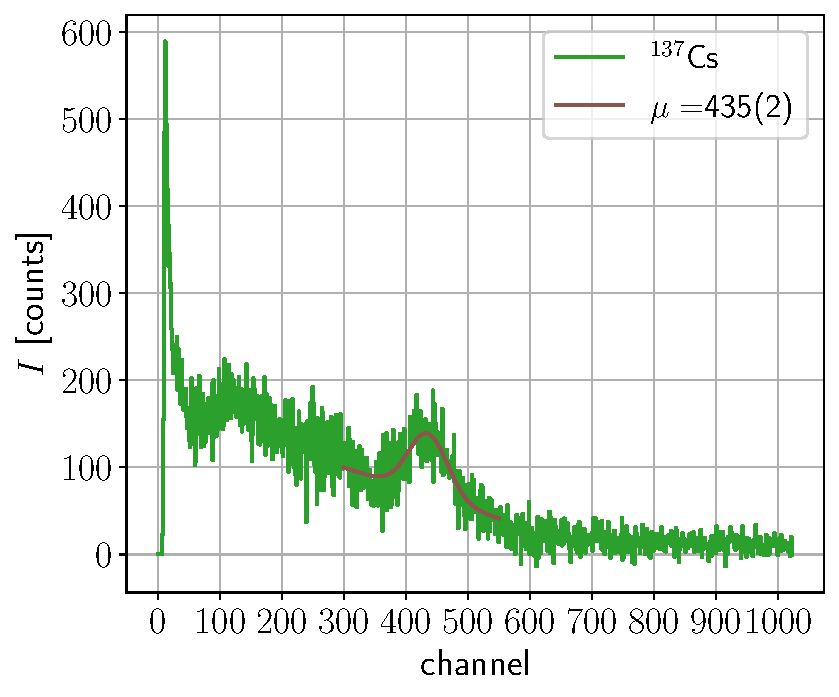
\includegraphics[width=\textwidth]{measurements/NIM/2024-05-24/outD/outD_137Cs.pdf}
    \caption{\label{sfig:NIM_137Cs}$^{137}$Cs, $A=23.139$ kBq.}
  \end{subfigure}
  \caption{\label{fig:NIM_spectra}Spectra measured with a Timing Filter Amplifier and Analog to Digital Converter NIM modules. The $x$ axis measures channels since the ADC creates a histogram based on pulse area. Each graph features the centroid of the Gaussian fitted to each peak.}
\end{figure}

\begin{figure}[H]
  \begin{subfigure}[t]{\textwidth}
    \centering
    \includegraphics[width=.98\textwidth]{measurements/NIM/2024-05-24/outD/LYSO_calibration.pdf}
    \caption{\label{sfig:NIM_LYSO_calibration}LYSO calibration from NIM modules data. Obtained by fitting gaussian functions to the main peaks shown in Fig \ref{sfig:NIM_22Na} to \subref{sfig:NIM_137Cs}.}
  \end{subfigure}
  \medskip
  \begin{subfigure}[t]{\textwidth}
    \centering
    \includegraphics[width=.98\textwidth]{measurements/NIM/2024-05-24/outD/Calibrated_spectrum.pdf}
    \caption{\label{sfig:NIM_LYSO_calibrated_spectrum}Calibrated spectrum obtained from the channel-energy conversion shown in \subref{sfig:NIM_LYSO_calibration}.}
  \end{subfigure}
  \caption{\label{fig:NIM_calibration}Gamma-ray spectra obtained with NIM modules.}
\end{figure}

Notably, this new calibration does not result in the prediction of negative energies, like in the case of the RTO6 oscilloscope, despite the various flaws in these spectra.